\documentclass[11pt,a4paper]{article}

\usepackage[utf8]{inputenc}
\usepackage[spanish]{babel}
\usepackage{graphicx}
\usepackage{amsmath}
\usepackage[left=3cm,top=2.5cm,right=3cm,bottom=2.5cm]{geometry} 
\usepackage{amsfonts}


\author{José Luis Nunes - 4.213.264-9 \\ Matías Tailanián - 4.555.937-1}
\title{Int. al reconocimiento de patrones - Informe de avances}
\date{}


\begin{document}
\maketitle

\section{Breve resumen del proyecto y su objetivo}

El objetivo principal del proyecto es la investigación en técnicas que permitan contribuir con la predicción de fertilidad de rodeo lechero y la calidad de la carne integrando técnicas de reconocimiento de patrones sobre datos de alta dimensión.\\

A lo largo de los últimos años varios grupos de Facultad de Veterinaria han creado bases de datos con información fenotípica y molecular relacionada con la calidad cárnica y la fertilidad bovina aplicada a la producción lechera. Este análisis requiere el relevamiento masivo de datos y su procesamiento en forma exhaustiva y eficiente. \\

\section{Estado actual}
\subsection{Bases de datos}

Contamos con dos bases de datos, una basada en las características fenotípicas y genotípicas mas relevantes respecto a la producción de leche y fertilidad del ganado bovino. Y la otra basada en las características fenotípicas y genotípicas que corresponden a la calidad de la carne en ganado bovino.\\

Estas bases fueron realizadas por expertos vinculados a los temas que ambas refieren, veterinarios, agrónomos y genetistas. Su lectura e interpretación no resulta para nada sencillo, es por esa razón que se realizaron dos reuniones con la Dr. Ana Meikle, encargada de la investigación que llevó a cabo la base asociada a la producción de leche y fertilidad del ganado bovino. En ambas reuniones se buscó depurar la base con el fin de quitar información repetida y no relevante para el estudio. También se estableció un orden de relevancia en las características fenotípicas.\\

Una vez establecida la base de datos con la cual vamos a trabajar nos dispusimos a emular la última investigación realizada con dicha base y los resultados obtenidos. La investigación se baso en análisis estadísticos, utilizando el software de análisis estadístico WEKA \cite{bib:weka}.

\subsection{Primeras pruebas}
Como primer acercamiento al procesamiento de los datos, se confeccionó un archivo \emph{.arff} con solamente las características que a priori son más relevantes para ser introducidas en WEKA y realizar un primer análisis de la situación.\\

Las características utilizadas son las siguientes:
\begin{itemize}
	\item CC: Condición corporal al momento del parto. La condición corporal es una medida del 1 al 5 que otorga el veterinario basándose en diferentes aspectos de la situación física del animal. 3 es lo óptimo, 1 corresponde a un animal ``flaco'' y 5 a un animal ``gordo''.
	\item CC30: Condición corporal a los 30 días del parto.
	\item CC45: Condición corporal a los 45 días del parto.
	\item CC60: Condición corporal a los 60 días del parto.
	\item CC75: Condición corporal a los 75 días del parto.
	\item CC90: Condición corporal a los 90 días del parto.
	\item LACTANCIA: Cantidad de ciclos de lactancia atravesador por el animal.
	\item ANESTRO: Tiempo en días entre el parto y el ``Reinicio''. El ``Reinicio'' se da cuando la progesterona supera un cierto umbral, indicando que el animal vuelve a estar ciclando.
	\item EDAD: Edad en meses del animal al día del parto.
	\item IIP: Intervalo en días entre los últimos 2 partos. Válido solo para animales multíparos.
	\item SECADO: Cantidad de días que pasan entre que se le deja de sacar leche a la vaca hasta que la vaca vuelve a parir.
	\item P4: Nivel de progesterona.
	\item SERVICIOS: Cantidad de inceminaciones realizadas para lograr la preñez.
	\item P100: Cantidad de litros de leche en 100 días.
\end{itemize}

Se consideran 3 clases, correspondientes a los distintos genotipos: AA, AB y BB.\\

Las distribuciones para cada clase, por característica se muestran en la figura \ref{fig:caracteristicas}.

\begin{figure}
	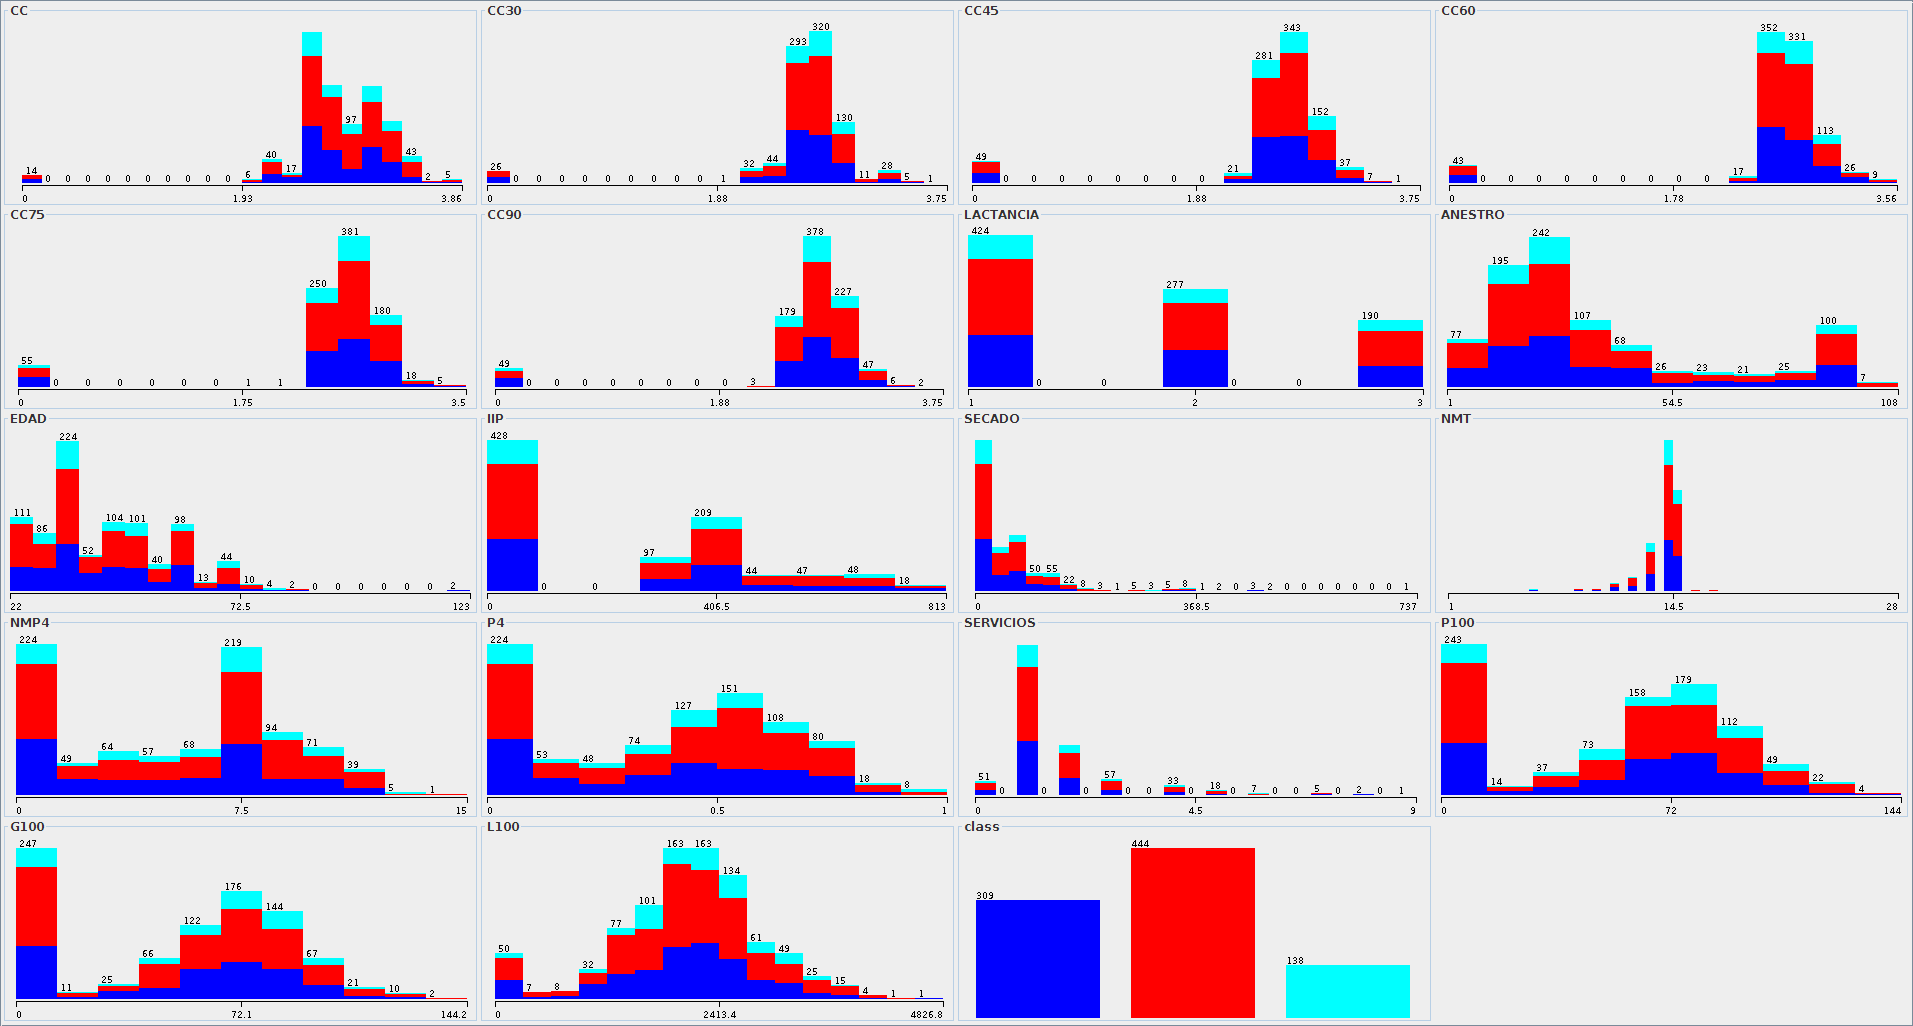
\includegraphics[width=1\textwidth]{./pics/caracteristicas.png}
	\caption{Distribución de características por clase.}
	\label{fig:caracteristicas}
\end{figure}

Como parte de las primeras pruebas se corrieron algunos algoritmos de clasificación:
\subsubsection*{Naive Bayes}
\begin{verbatim}
Correctly Classified Instances         329               36.9248 %
Incorrectly Classified Instances       562               63.0752 %
\end{verbatim}

\subsubsection*{C4.5}
\begin{verbatim}
Correctly Classified Instances         360               40.404  %
Incorrectly Classified Instances       531               59.596  %
\end{verbatim}

\subsubsection*{Attribute Selected Classifier - Cfs Subset Eval - Best First}
\begin{verbatim}
Correctly Classified Instances         444               49.8316 %
Incorrectly Classified Instances       447               50.1684 %
\end{verbatim}

Como se puede observar se obtuvieron unos resultados preliminares asombrosamente malos, por lo que habrá que buscar otras técnicas o algoritmos.

\section{Trabajo a futuro}

Se plantean 2 etapas de trabajo:
\begin{itemize}
	\item La primera consiste en estudiar los resultados reportados en el informe y reproducirlos. 
	\item La segunda etapa se basa en la investigación e implementación del algoritmo REML (Restricted Maximum Likelihood) \cite{bib:REML}.
\end{itemize}

\begin{thebibliography}{99}
\bibitem{bib:weka}Mark Hall, Eibe Frank, Geoffrey Holmes, Bernhard Pfahringer, Peter Reutemann, Ian H. Witten (2009); The WEKA Data Mining Software: An Update; SIGKDD Explorations, Volume 11.
\bibitem{bib:REML}Meyer, K. (2007). WOMBAT – A tool for mixed model analyses in quantitative genetics by REML, J. Zhejiang Uni.
\end{thebibliography}


\end{document}